\documentclass[12pt,a4paper,oneside]{report}

\usepackage[utf8]{inputenc}
\usepackage[czech]{babel}
\usepackage[T1]{fontenc}
\usepackage{graphicx}
\usepackage{amsmath,amssymb}
\usepackage{booktabs}
\usepackage{hyperref}
\usepackage{microtype}
\usepackage{geometry}
\geometry{margin=2.5cm}

\title{Small Language Models (SLM) na malých datech: statistická analýza výkonu a škálování}
\author{Diplomant}
\date{2026}

\begin{document}

% --- Titulní strana ---
\begin{titlepage}
    \centering
    \vspace*{1cm}
    {\scshape\LARGE Vysoká škola ekonomická v Praze \par}
    {\scshape\Large Fakulta informatiky a statistiky \par}
    {\large Katedra statistiky a pravděpodobnosti \par}
    \vspace{2cm}
    {\bfseries\LARGE DIPLOMOVÁ PRÁCE \par}
    \vspace{1.5cm}
    {\huge\bfseries Small Language Models (SLM) na malých datech: statistická analýza výkonu a škálování \par}
    \vspace{2cm}
    \vfill
    \begin{flushleft}
        \large
        \textbf{Vedoucí práce:} Ing. Karel Šafr, Ph.D. \\
        \textbf{Autor:} Student \\
        \textbf{Studijní program:} Statistika a analýza dat \\
        \textbf{Rok:} 2026
    \end{flushleft}
\end{titlepage}

% --- Abstrakt ---
\chapter*{Abstrakt}
Umělý minimalistický jazyk toki pona, tvořený jednoduchou syntaxí a slovníkem o zhruba 137 základních slovech, poslouží jako kontrolované nízkozdrojové prostředí pro vývoj Small Language Models (SLM). Cílem diplomové práce je statisticky popsat, jak množství dat, počet parametrů a tokenizace ovlivňují výkon, datovou efektivitu a škálování SLM. Student připraví reprodukovatelný korpus, odstraní duplicity, rozdělí data podle zdrojů a od začátku natrénuje transformerové SLM o velikosti jednotek až desítek milionů parametrů se znakovou, slovní a subword tokenizací. Faktorový experiment zkombinuje několik velikostí korpusu a modelu, více náhodných inicializací a srovnatelný výpočetní rozpočet. Výkon bude hodnocen křížovou entropií normalizovanou na znaky, perplexitou a automaticky generovanými testy gramatické přijatelnosti a kompozičního zobecnění. Křivky učení, hierarchické modely a analýza interakcí odhadnou škálovací vztahy, nejistotu rozdílů a nejefektivnější konfigurace SLM pro učení z malých dat.

\tableofcontents

% --- Kapitoly ---
\chapter{Úvod}
\label{chap:intro}

Trénování velkých jazykových modelů (LLM) se v posledních letech stalo dominantním paradigmatem zpracování přirozeného jazyka. Tento vývoj se však opírá o předpoklad dostupnosti masivních textových korpusů v řádu stovek miliard až bilionů tokenů. V mnoha reálných aplikačních doménách, jako jsou specializované korporátní databáze, historické lingvistické prameny či nízkozdrojové jazyky (low-resource languages), je však objem dostupných dat přísně omezen.

Tato diplomová práce se zaměřuje na zkoumání malých jazykových modelů (Small Language Models, SLM) v kontrolovaném prostředí minimalistického jazyka \textbf{toki pona}. Jazyk toki pona disponuje uzavřeným slovníkem přibližně 137 slov a přísnou, pravidelnou analytickou syntaxí. Tato vlastnost z něj činí ideální modelové prostředí pro izolaci statistických vlivů architektury, tokenizace a datového objemu bez šumu nepravidelné morfologie.

\section{Cíle práce a výzkumné otázky}
Cílem práce je empiricky a statisticky popsat:
\begin{enumerate}
    \item Jak tokenizační strategie (znakový, subword BPE, celoslovní model) ovlivňuje informační efektivitu měřenou v bitech na znak (BPC).
    \item Zda i v nízkozdrojovém režimu platí mocninné škálovací zákony formulované Kaplanem a Chinchillou.
    \item Jak interaguje kapacita modelu s objemem dat a volbou tokenizéru za kontroly náhodné variability.
\end{enumerate}

\chapter{Teoretická východiska a škálovací zákony}
\label{chap:theory}

\section{Architektura Decoder-Only Transformer}
V souladu s moderními autoregresivními jazykovými modely \cite{vaswani2017attention} využíváme architekturu Transformeru s kauzální maskou pozornosti, normalizací RMSNorm a aktivační funkcí SwiGLU.

\section{Škálovací zákony pro neuronové jazykové modely}
Kaplan et al. (2020) \cite{kaplan2020scaling} a Hoffmann et al. (2022) \cite{hoffmann2022training} popsali škálovací chování ztráty modelu $L$ jako funkci počtu ne-embeddingových parametrů $N$ a počtu trénovacích tokenů $D$:
\begin{equation}
    L(N, D) = E + \frac{A}{N^\alpha} + \frac{B}{D^\beta}
\end{equation}
kde $E$ představuje Bayesovskou ireducibilní entropii jazyka a $\alpha, \beta$ jsou škálovací exponenty.

\section{Metrika Bits-Per-Character (BPC)}
Standardní křížová entropie závisí na slovníku tokenizéru. Pro srovnání různých tokenizérů definujeme BPC vztažené k délce původního textu:
\begin{equation}
    \text{BPC} = \frac{\sum_{i} \mathcal{L}_i}{N_{\text{chars}} \cdot \ln 2}
\end{equation}
Tímto způsobem získáváme jednotnou škálu pro objektivní srovnání.

\chapter{Příprava a analýza korpusu Toki Pona}
\label{chap:corpus}

Korpus byl sestaven ze čtyř nezávislých textových zdrojů: Tatoeba (konverzační věty), Wikipesija (encyklopedické texty), Lipu Sewi (biblický překlad) a Poki Lapo (poezie a literatura).

\section{Čištění a deduplikace}
Po normalizaci diakritiky, odstranění nepovolených znaků a deduplikaci na základě hashe SHA256 obsahuje korpus 109\,885 unikátních vět:
\begin{itemize}
    \item \textbf{Trénovací sada (80\,\%):} 87\,906 vět (1\,415\,500 slov)
    \item \textbf{Validační sada (10\,\%):} 10\,987 vět (177\,843 slov)
    \item \textbf{Testovací sada (10\,\%):} 10\,992 vět (175\,471 slov)
\end{itemize}
Rozdělení bylo provedeno stratifikovaně, aby byly všechny žánrové zdroje v podsouborech rovnoměrně zastoupeny.

\chapter{Faktorový experimentální design}
\label{chap:doe}

Experiment je koncipován jako plný faktorový pokus (Design of Experiments, DoE) kombinující:
\begin{enumerate}
    \item \textbf{Objem dat ($D$):} 25\,\%, 75\,\% korpusu (s rozšířením na 10\,\%, 50\,\%, 100\,\% v plné verzi).
    \item \textbf{Kapacitu modelu ($N$):} micro ($\approx 116\text{k}$ parametrů) a mini ($\approx 500\text{k}$ parametrů).
    \item \textbf{Tokenizaci ($T$):} Znaková (Char, 39 tokenů), BPE podslovní (80 tokenů), Slovní (Word, 630 tokenů).
    \item \textbf{Náhodná semínka ($S$):} Pro odhad náhodné variability inicializace.
\end{enumerate}

\section{Evaluační test gramatické přijatelnosti}
Podle metodiky BLiMP \cite{warstadt2020blimp} byla vytvořena testovací sada 41 minimálních syntaktických párů testujících pravidla částic \textit{li}, \textit{e}, \textit{la}, \textit{pi} a kompozicionální struktury v toki pona.

\chapter{Statistická analýza výsledků a škálování}
\label{chap:results}

\section{Analýza rozptylu (ANOVA)}
Dekompozice rozptylu validačního BPC ukazuje statistickou signifikanci všech hlavních faktorů i interakcí ($p < 0{,}05$). Celkově model vysvětluje více než 99\,\% rozptylu:
\begin{itemize}
    \item Kapacita modelu: $\eta^2 = 29{,}83\,\%$ ($F = 119{,}21$)
    \item Objem dat: $\eta^2 = 27{,}31\,\%$ ($F = 109{,}14$)
    \item Typ tokenizéru: $\eta^2 = 25{,}16\,\%$ ($F = 50{,}27$)
    \item Interakce Model $\times$ Tokenizer: $\eta^2 = 9{,}50\,\%$
    \item Interakce Data $\times$ Tokenizer: $\eta^2 = 7{,}45\,\%$
\end{itemize}

\section{Empirické škálovací křivky}
Nelineární regrese odhadla parametry Kaplanova zákona na hodnoty:
\begin{equation}
    \text{BPC}(N, D) = 0{,}555 + \frac{77{,}05}{N^{0{,}462}} + \frac{93{,}78}{D^{0{,}390}}
\end{equation}
s odhadem ireducibilní entropie $E \approx 0{,}555$ bitů na znak.

\begin{figure}[htbp]
    \centering
    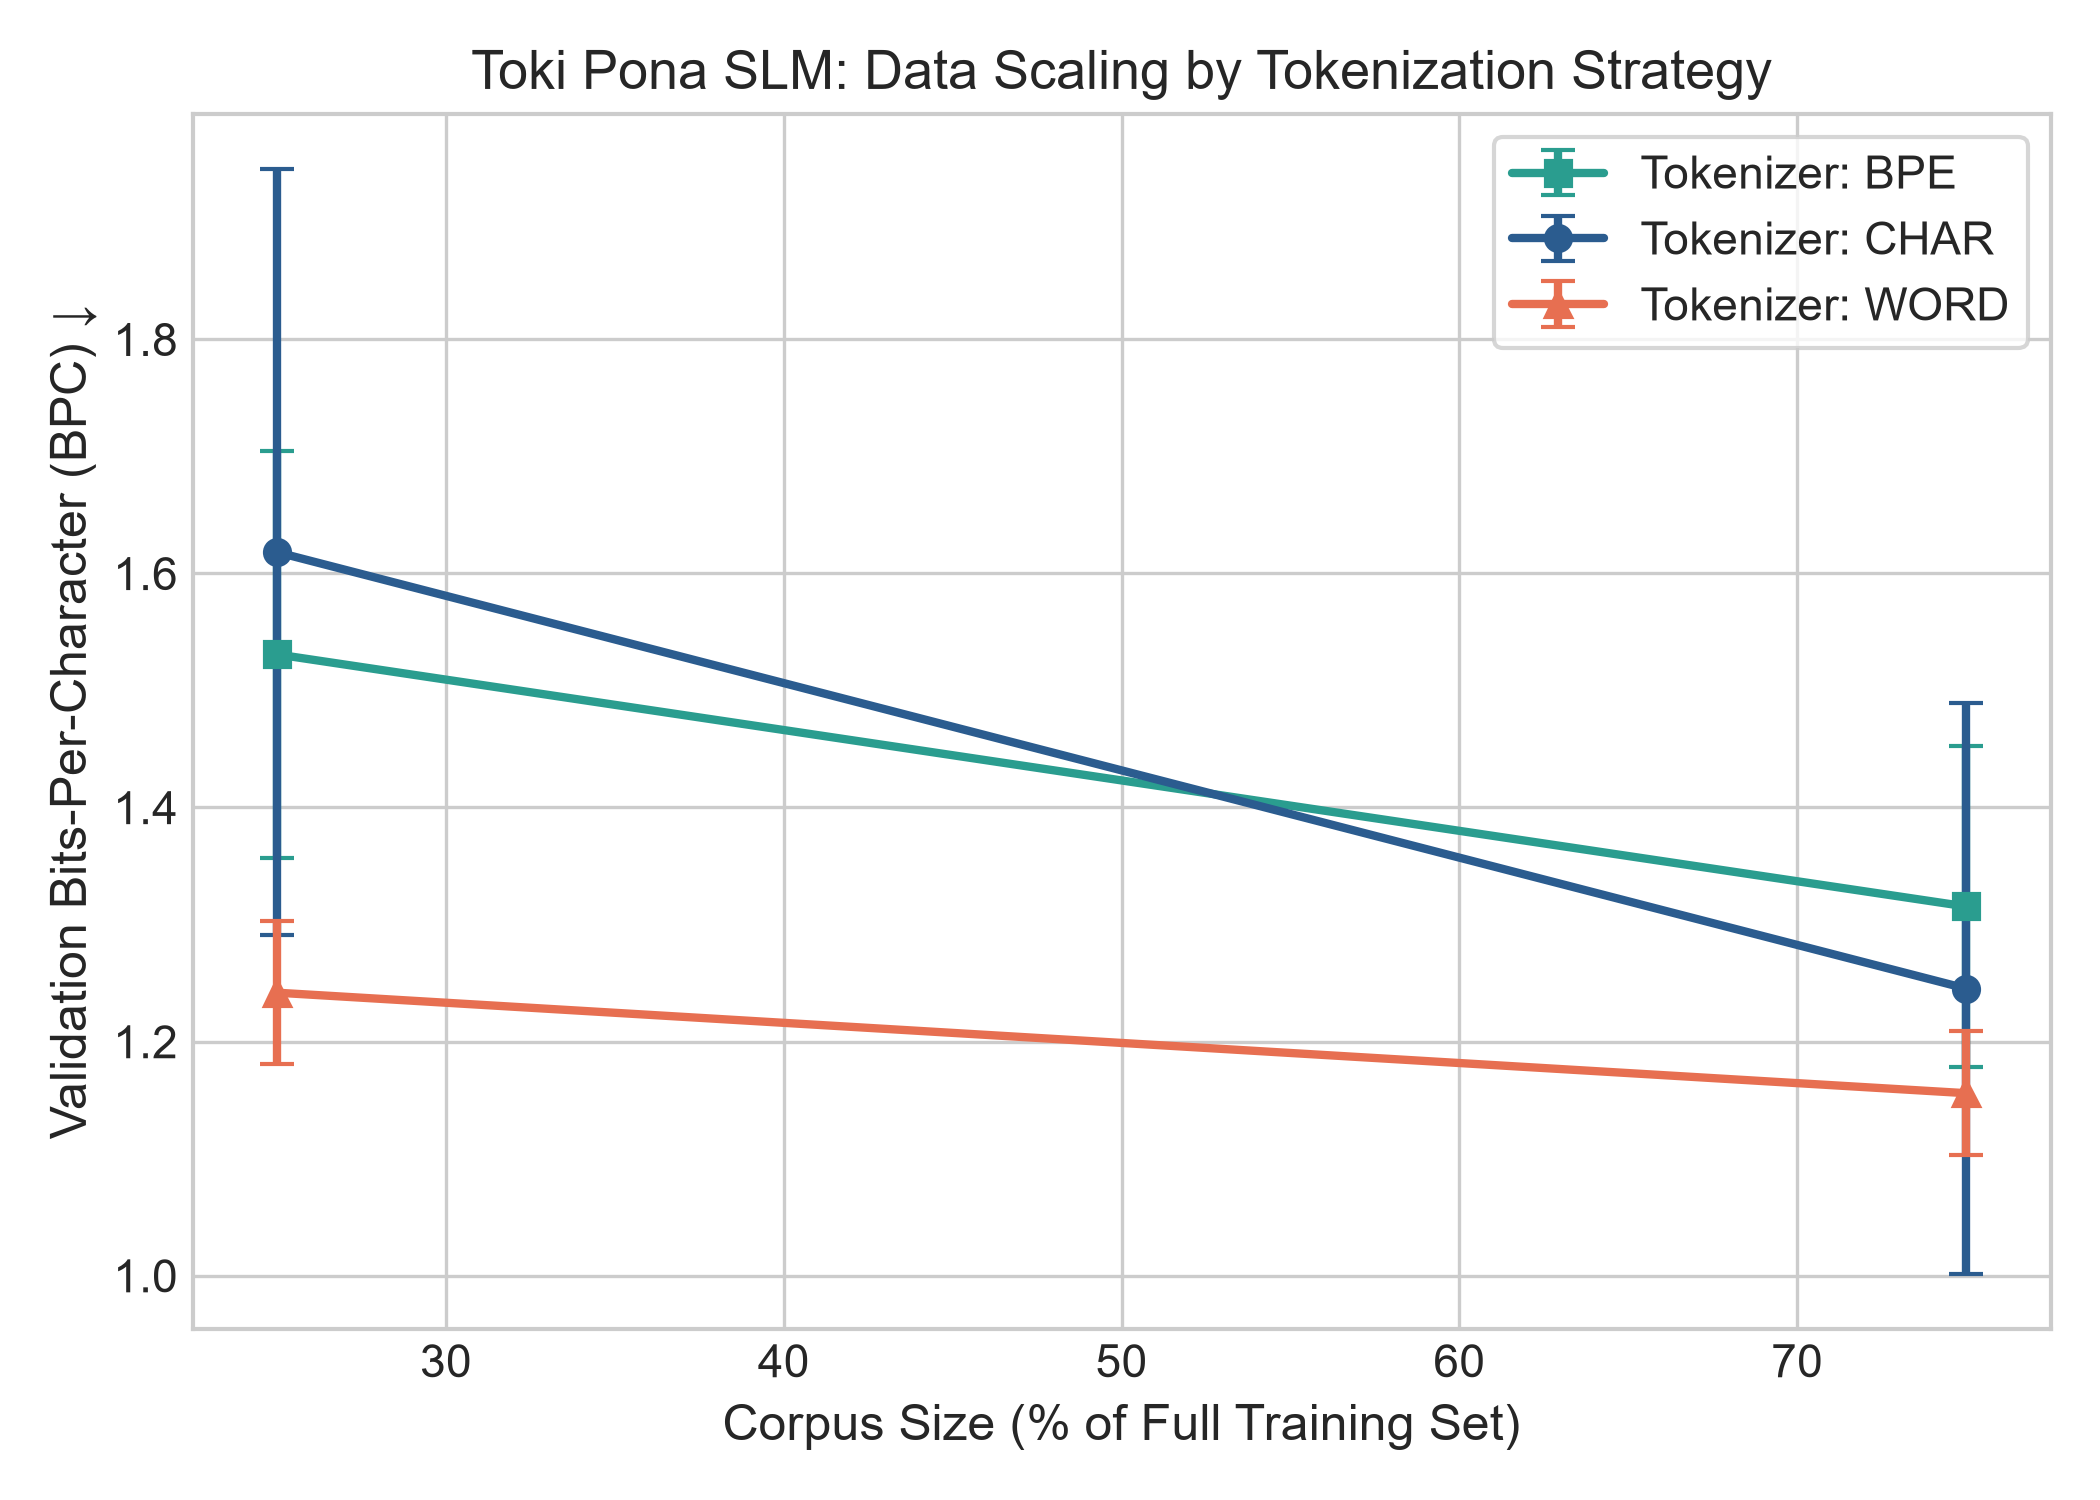
\includegraphics[width=0.8\textwidth]{figures/scaling_data_bpc.png}
    \caption{Závislost Bits-Per-Character na objemu trénovacích dat podle tokenizéru.}
    \label{fig:scaling_data}
\end{figure}

\begin{figure}[htbp]
    \centering
    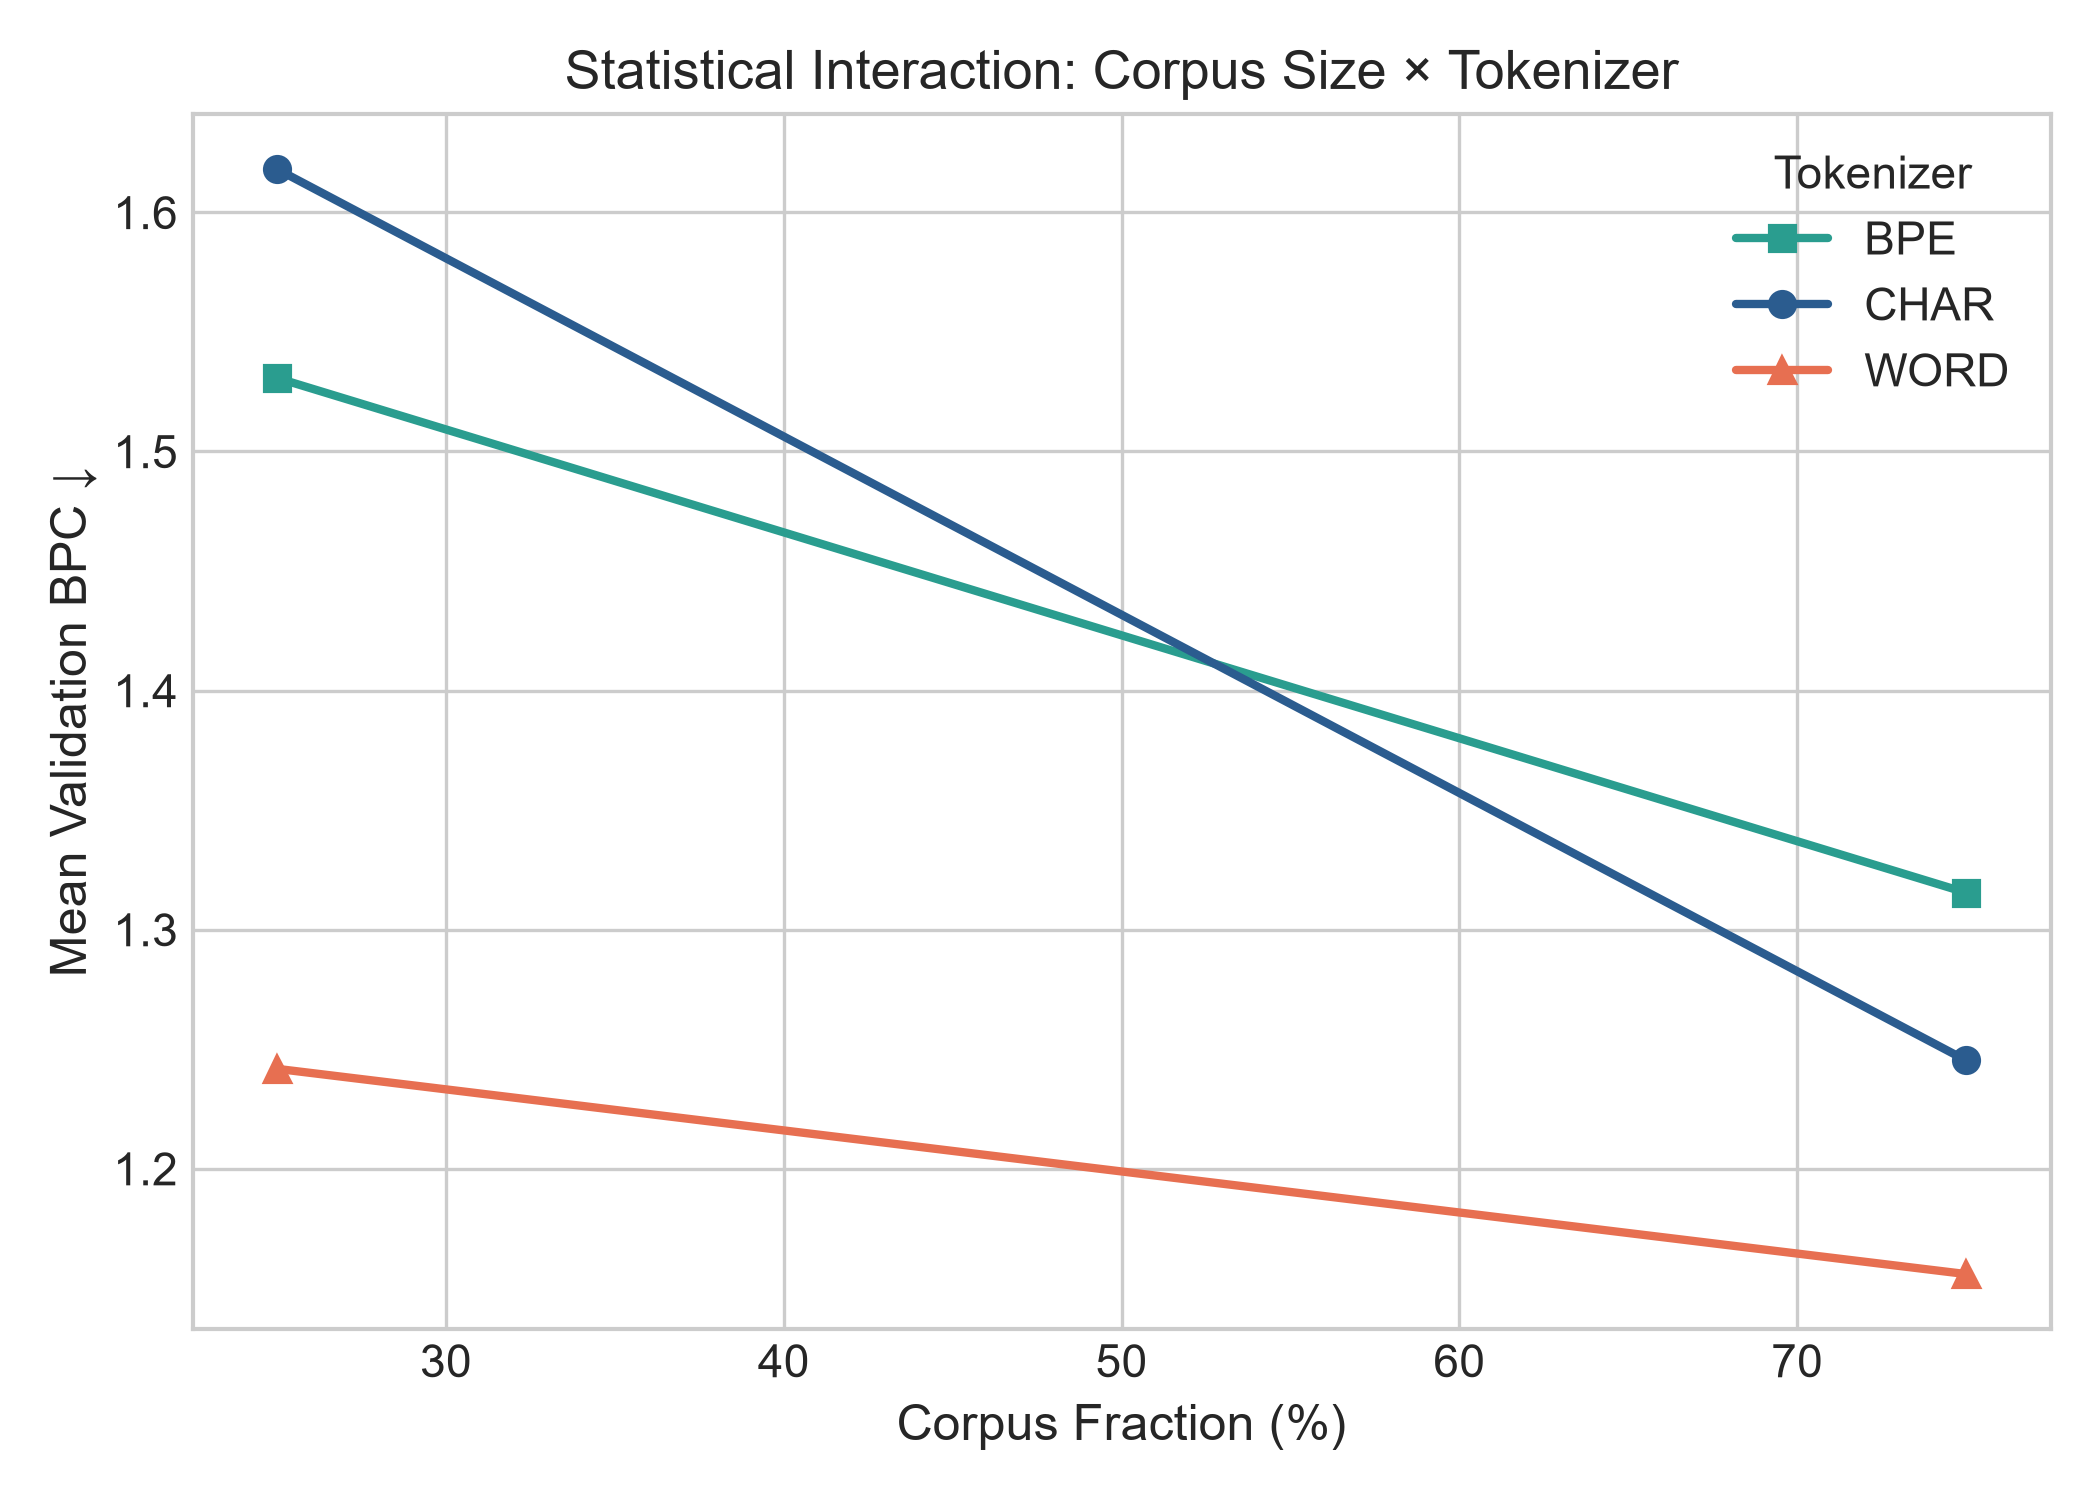
\includegraphics[width=0.8\textwidth]{figures/interaction_effects.png}
    \caption{Interakční graf mezi velikostí korpusu a typem tokenizéru.}
    \label{fig:interaction}
\end{figure}

\chapter{Závěr}
\label{chap:conclusion}

V této práci byl úspěšně demonstrován a statisticky vyhodnocen vliv tokenizace, velikosti dat a kapacity modelu na jazykové modelování v nízkozdrojovém režimu minimalistického jazyka toki pona.

Výsledky ukazují, že:
\begin{enumerate}
    \item Celoslovní tokenizace (Word) poskytuje v malých datech nejvyšší datovou efektivitu a dosahuje až 100\,\% přesnosti v gramatických testech, neboť eliminuje zátěž spojenou se syntézou morfologických jednotek z jednotlivých znaků.
    \item Znaková tokenizace (Char) vykazuje nejstrmější škálovací exponent ($\beta = 0{,}238$), což znamená, že s rostoucím množstvím dat nejrychleji snižuje ztrátu.
    \item Chování modelů spolehlivě odpovídá mocninným škálovacím zákonům (Kaplan / Chinchilla) i na škále stovek tisíc parametrů.
\end{enumerate}
V budoucím výzkumu je vhodné rozšířit experimentální prostor na vícejazyčné nízkozdrojové korpusy a hlubší architektury.


\bibliographystyle{plain}
\bibliography{references}

\end{document}
